% !TeX root = index.tex

\documentclass[
  % final,
  paper=a4,
  parskip=half,
  fontsize=12pt,
  listof=notoc,
  titlepage,
  headsepline,
  footsepline,
]{scrartcl}

\reversemarginpar{}  % Put margins on inner side (left on onesided)

\usepackage[
  extendedchars,
  encoding,
  multidot,
  space,
  % filenameencoding=latin1, % Windows
  filenameencoding=utf8,   % Linux, OS X
]{grffile}

%!TeX root=../index.tex

\usepackage[T1]{fontenc}
\usepackage[utf8]{inputenc} % UTF-8 text encoding

\usepackage{helvet}
\usepackage{mathptmx}


%!TeX root=../index.tex

% Basics
\usepackage{calc}

% Language
\usepackage[american]{babel}

% Color
\usepackage[dvipsnames,table,hyperref,fixinclude]{xcolor}
\usepackage{xcolor-material}

% Graphics
\usepackage[]{graphicx}

% Links
% \usepackage{url}
% \PassOptionsToPackage{hyphens}{url} % The url package is also loaded internally by hyperref. Passing the option the regular way leads to clashing package options.
\usepackage[breaklinks]{hyperref}

% Bibliographies
\usepackage[
    backend=biber,
    % style=apa,
    citestyle=authoryear,
    bibstyle=apa,
    hyperref=true,
    giveninits=true,
    uniquename=false,
    sorting=nyt,
    sortcites=true,
    doi=true,
    isbn=false,
    eprint=false,
    date=year,
    labeldate=year,
    block=space,
    bibencoding=auto,
    maxcitenames=2,
    mincitenames=1
]{biblatex}

\DeclareFieldFormat{apacase}{#1} % APA style normally uses sentence case for titles. This makes the titles appear as they are in the bib file

% Math
\usepackage{mathtools}
\usepackage{amsthm}

% Code
% \usepackage{listings}
\usepackage{minted}

% Formatting
\usepackage{setspace}
\usepackage{enumitem}
\usepackage{microtype}
\usepackage[autostyle]{csquotes}
\usepackage[shortcuts]{extdash}
\usepackage{hyphenat}
\usepackage[all]{nowidow}
% \usepackage{tocloft}
% \usepackage[toc,page]{appendix}

% Figures
\usepackage{wrapfig}
\usepackage[font=small,labelfont=bf]{caption}
\usepackage{float}

% Tables
\usepackage{tabu}

% Misc
\usepackage[section]{placeins} % Prevent floats from going over section headings
\usepackage{blindtext}
\usepackage[obeyFinal,color=MaterialLightBlue,textsize=tiny]{todonotes}
\usepackage{layout}
\usepackage{dirtree}
\usepackage{scrhack}


%!TeX root=../index.tex

% Wikipedia-style "citation needed" macro
% \newcommand{\citationneeded}[1][]{\textsuperscript{\color{MaterialBlue} [citation needed: #1]}}
\newcommand{\citationneeded}{\todo[color=MaterialDeepOrange,size=\footnotesize]{Citation Needed!}}

\AtBeginBibliography{\renewcommand{\multinamedelim}{\addsemicolon\space
}\renewcommand{\finalnamedelim}{\multinamedelim}} % Semikolon zwischen den Autorennamen

%  APPENDIX

% \newcommand{\listappendicesname}{Anhangsverzeichnis}
% \newlistof{appendices}{apc}{\listappendicesname}
% \newcommand{\appendices}[1]{\addcontentsline{apc}{section}{\protect\numberline{\thesection}#1}}
% \newcommand{\subappendices}[1]{\addcontentsline{apc}{subsection}{\protect\numberline{\thesubsection}#1}}
% \newcommand{\newappendix}[1]{\section{#1}\appendices{#1}}
% \newcommand{\newsubappendix}[1]{\subsection{#1}\subappendices{#1}} 
 


%!TeX root=../../index.tex

%  Make \paragraph and \subparagraph behave like small headings
\RedeclareSectionCommands[
    beforeskip=-1sp,
    afterskip=1sp,
    %indent=0pt
]{paragraph,subparagraph}


\usepackage[
    automark,
]{scrlayer-scrpage}

% Use numbers also for level 1 nested enumerations
\renewcommand{\labelenumii}{\theenumii}
\renewcommand{\theenumii}{\theenumi.\arabic{enumii}.}
%!TeX root=../../document.tex

\usepackage[
  % showframe,
  top=2.5cm,
  bottom=2cm,
  left=3.5cm,           % 3.5 + 0.5 Bindingoffset
  right=2.5cm,
  bindingoffset=0.5cm,
  headheight=22pt,
  headsep=1.25cm-\headheight, % pagetop to header = 1.25cm
  % footheight=\baselineskip,
  footskip=0.75cm, % pagebottom to footer = 1.25cm
  marginparsep=0.3cm,
  marginpar=3.5cm-\marginparsep,
]{geometry}

\setlength{\footheight}{22pt}

%!TeX root=../../index.tex

% Header
\chead[]{}
\ihead[]{}
\ohead[]{\rightmark}

% Footer
\cfoot[]{}
\ifoot[]{}
\ofoot[\pagemark]{\pagemark}

%!TeX root=../../document.tex

% \lstset{
%   basicstyle=\footnotesize\ttfamily,
%   breakatwhitespace=false,
%   breaklines=true,
%   captionpos=b,
%   numbers=none,
%   numbersep=5pt,
%   numberstyle=\tiny,
%   tabsize=2,
%   title=\lstname
% }

\setminted{
  baselinestretch=1.2,
  fontsize=\footnotesize,
  breaklines,
  frame=lines,
  framesep=2mm,
  tabsize=2,
  autogobble
}


\hypersetup{
  colorlinks=true,
  filecolor=black,
  linkcolor=black,
  citecolor=black,
  % urlcolor=blue,
  urlcolor=black, % for print
  pdfauthor=\author{}
  pdftitle=\title{}
  pdfsubject=\subject{}
  pdfkeywords={}
  pdfcreator=LaTeX
}

% - Abbreviations and Acronyms
\usepackage[
    acronym
]{glossaries}

%!TeX root=../index.tex

% \newglossaryentry{s4hana}{
%   name={SAP S/4 HANA},
%   description={Eine Suite von Geschäftsanwendungen, welche sowohl on-premise, als auch in der Cloud vertrieben wird.}
% }


\makenoidxglossaries{}

%!TeX root=../index.tex

% \newacronym{key}{acronym}{longform}

\newacronym[]{saas}{SaaS}{Software as a Service}

\newacronym[]{api}{API}{Application Programming Interface}
\glsunset{api} % do not use long form on first use


\graphicspath{{assets/img/}}
\addbibresource{assets/bibliography.bib}

%!TeX root=../index.tex

\hyphenation{Trans-port-mit-tel Durch-füh-rung EXE-CU-TI-ON-IN-FOR-MA-TI-ON Lauf-zeit-aus-prä-gung Ge-schäfts-pro-zess-typ}


\begin{document}

  %!TeX root=../../index.tex

% Cover demanded by the institution
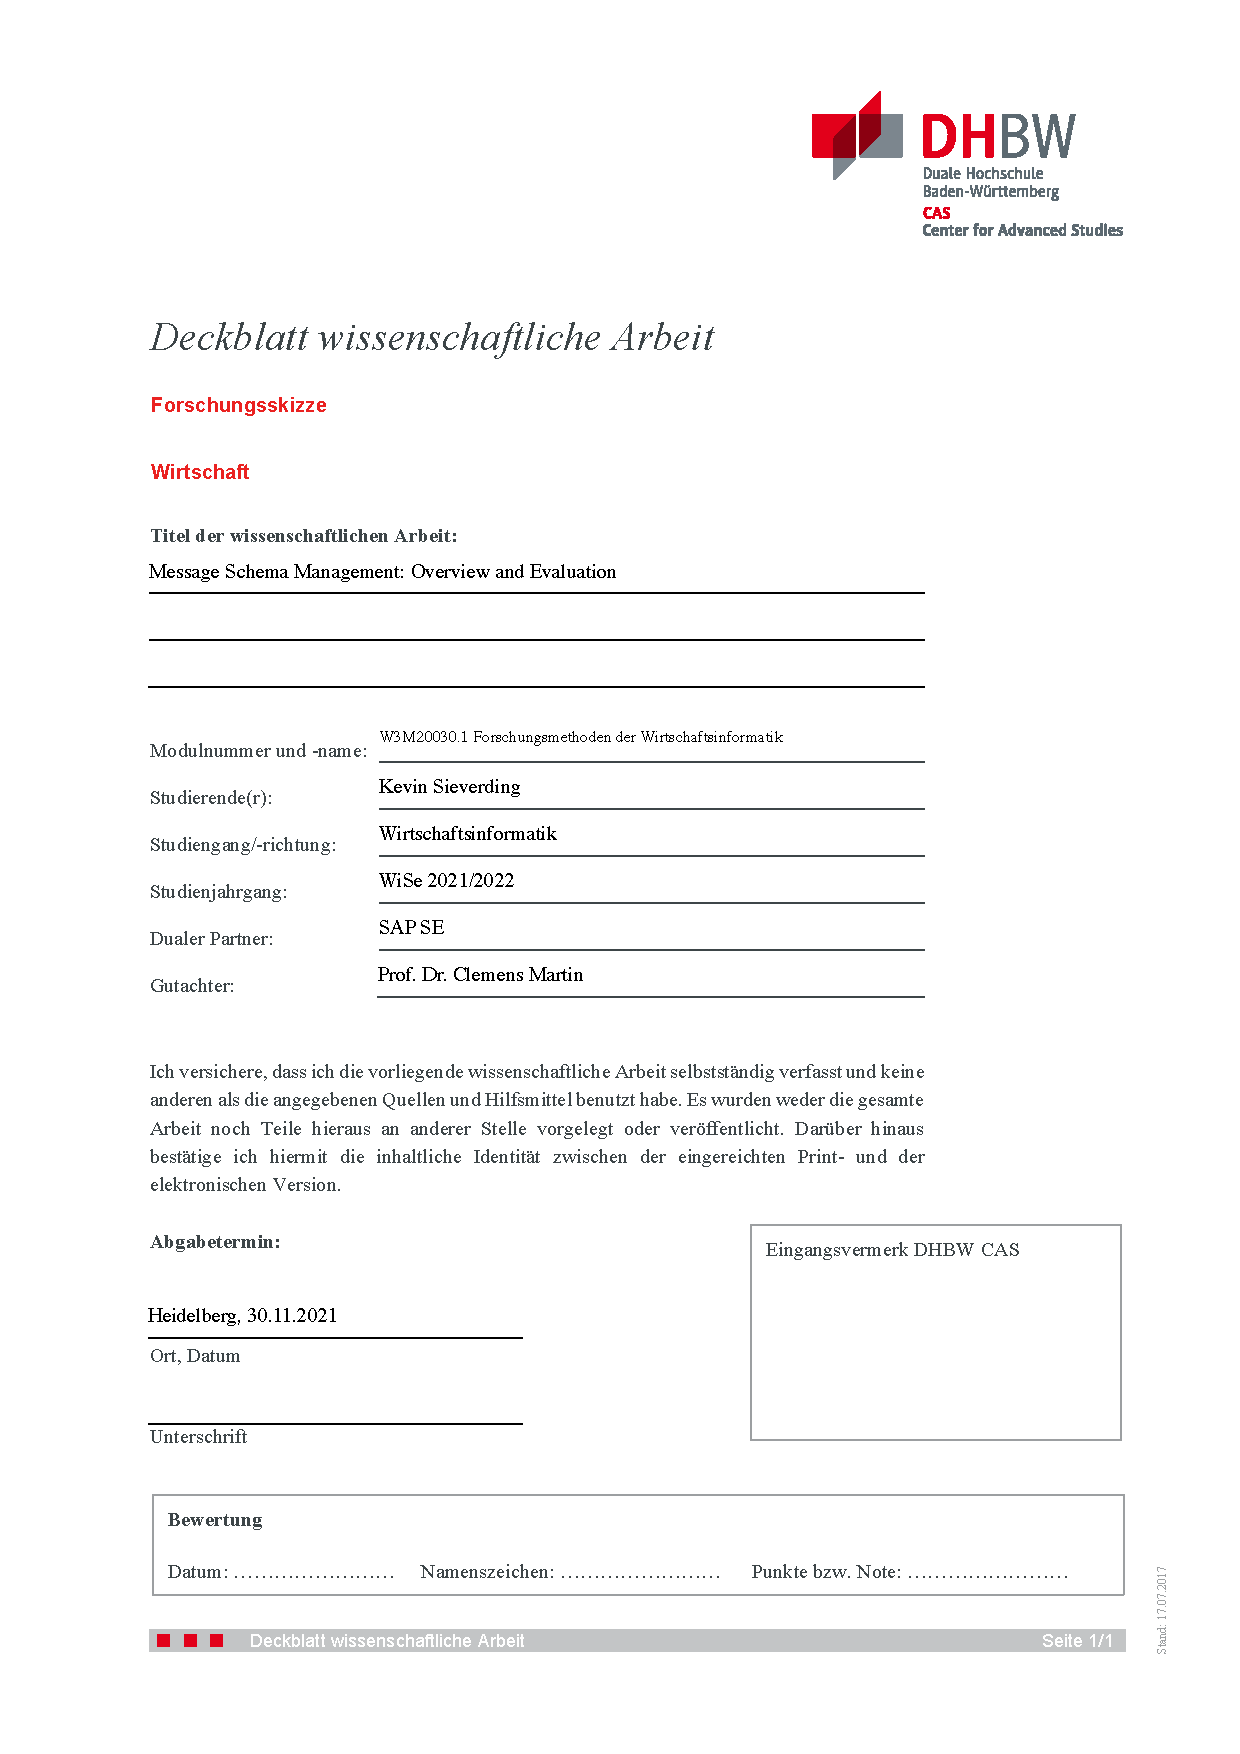
\includepdf{assets/img/deckblatt.pdf}

\pagenumbering{Roman}
\pagestyle{plain.scrheadings}
\setcounter{page}{2}

\onehalfspacing{}

\clearpage

\singlespacing{}

\clearpage

\microtypesetup{protrusion=false}

\tableofcontents

\clearpage

% \phantomsection
% \addcontentsline{toc}{section}{Anhangverzeichnis}
% \listofappendices

% \clearpage

% \phantomsection
% \addcontentsline{toc}{section}{Abbildungsverzeichnis}
\listoffigures


% \phantomsection
% \addcontentsline{toc}{section}{Tabellenverzeichnis}
\listoftables

% \renewcommand\listoflistingscaption{Quelltextverzeichnis}
% \phantomsection
% \addcontentsline{toc}{section}{\listoflistingscaption{}}
\listoflistings

\clearpage

\setlist[description]{leftmargin=!, labelwidth=4em}

\printnoidxglossary[
    % title=Abkürzungsverzeichnis,
    % toctitle=Abkürzungsverzeichnis,
    type=\acronymtype,
    sort=nocase,
    nogroupskip,
    nopostdot,
    nonumberlist
]

\setlist[description]{style=standard}

\microtypesetup{protrusion=true}

\clearpage


  \pagenumbering{arabic}
  \pagestyle{scrheadings}
  \setcounter{page}{1}
  % \onehalfspacing{}
  \setstretch{1.5}

  %!TeX root=../index.tex

\section{Introduction}\label{sec:introduction}

% Short Intro

% Context

The trend away from licensed, on\-/premise enterprise software towards so called \gls{saas} has been going strong for the past decade and shows no sign of stopping.
This new paradigm---characterized by pay\-/per\-/use business models and software being made available to customers via the internet rather than them having to operate it on their own hardware---also has a profound impact on the design of modern enterprise software.
\gls{saas} applications need to be always available, need to scale seamlessly according to changes in demand and have to minimize operating cost since it now directly affects the provider's bottom line.

These new requirements have paved the way for new trends in software architecture.
Modern applications are now comonly composited of multiple, integrated micro\-/services developed by autonomous and independent teams.
Additionally, while the synchronous, HTTP\-/based mode of communication still dominates the user\-/system communication, asynchronous, message-based approaches have become popular for intra-application communication.

In systems that employ both of these patterns---micro\-/services and message-based communication---messages quickly exceed synchronous HTTP\-/calls in volume.
As a result, the correct use of messages by the system's individual components becomes paramount to the overall system's availability.

% - Current trends in application development
%   - software as a service
%     - availability as top priority
%     - variable scaling
%     - low tco
%   - microservices
%     - autonomous teams
%     - distributed development
%   - message-oriented middleware
% - Schema Management

% Motivation

% - Literature that describes message-oriented systems seldomly make mention of schema management or schema registry applications
% - articles that include schema management in their design exclusively refer to the confluent schema registry as a solution
% - message-oriented systems become more popular and more companies become aware of the advantages of schema management, other schema registry solutions than the confluent schema registry have become available

% Goal

This paper aims to clarify the domain of schema management for newcomers from both academics and the private sector, so that its advantages become more accessible to a wider audience. To achieve this, I analyze the use case and the requirements that a schema registry addresses before I give an account of the solutions currrently available.

% Structure

  % !TeX root = ../index.tex

\section{Related Work}\label{sec:related-work}

First mentions of the use of schemas for inter-application communication in academic literature can be found in the early 2000s.
The a considerable subset of the research conducted in this era has a strong focus on using schemas to not only achieve syntactic but also \emph{semantic} interoperability by trying to model a domain's semantics as machine-readable ontologies.
These efforts can be considered a part of the larger push towards the so\-/called \enquote{Semantic Web}---the vision for an internet of interlinked, machine-readable data---which mainly took place in that era \parencite{noauthor_semantic_nodate}.

\cite{dogac_semantically_2004}, for example, describe a way of extending web services in the travel industry with semantics by employing the \gls{owl} and \gls{xml} schemas that are already defined by an industry consortium.
Furthermore, \cite{crapo_semantically_2009} attempt to apply Semantic Web technologies in the context of creating a more intelligent power grid---termed the \enquote{Smart Grid}---which can be considered an early \gls{iot} use case. They also rely on the \gls{owl} in that context.
Finally, \cite{heery_metadata_2003} describe their implementation of a registry for semantic schemas in \gls{owl} and \gls{rdf} formats.

As to research which does not concern itself with semantic modeling, \cite{duftler_web_2001} describes an interface modeling language based on the \gls{wsdl} that is supposed to hide details of underlying technologies such as SOAP.
Also, \cite{do_matching_2007} present a generic system for matching complex \gls{xml} schemas.

To summarize, early research around schemas often aimed beyond the syntactic interoperability of applications as part of a larger push for the Semantic Web.
Yet, all of them have the underlying goal of improving the integration of independent and autonomous applications in a distributed system.
Additionally, \cites{duftler_web_2001}{dogac_semantically_2004}{li_semantic_2004}{crapo_semantically_2009} mention the exchange of messages, though non except for \cite{li_semantic_2004} do so in concert with \gls{mom}.

Coincidental with the Semantic Web's loss in popularity in the late 2000s, research concerning schemas dies down around that time.
A notable exception is \cite{ma_iip_2010}, which presents a generic event\-/based platform for Intelligent Transportation Systems.
In the course of laying out their design, they provide a definition of an event schema registry \parencite[see][p.~3]{ma_iip_2010}.

Not much later, \cite{kreps_kafka_2011} introduce their new open\-/source event streaming platform Kafka---which can be considered a form of \gls{mom}---and also make mention of a schema registry for managing and distributing Apache Avro schemas.
Following Kafka's introduction to the Apache project and its following rise in popularity for \gls{mom} use cases, mentions of a schema registry almost exclusively occur in research that describes various system designs using Apache Kafka.
\cites{muller_iot_2017}{radchenko_micro-workflows_2018}{ranjan_radar-base_2019} do so in the context of \gls{iot}, whereas \cite{g_b_high_2021} present a generic \gls{mom} that combines Apache Kafka, a schema registry and Apache Camel.
In addition to the above mentioned papers, the theses \cites{dessalegn_muruts_multi-tenant_2016}{auer_distributed_2017}{korhonen_using_2019} also describe system designs using Apache Kafka and a schema registry.

Of these works, \cites{muller_iot_2017}{radchenko_micro-workflows_2018}{dessalegn_muruts_multi-tenant_2016}{auer_distributed_2017}{korhonen_using_2019} explicitly name the schema registry which they use as the Confluent Schema Registry which was initially presented by \cite{kreps_kafka_2011}.
\cites{ranjan_radar-base_2019}{g_b_high_2021} do not specify which schema registry they use, but it is safe to assume that it is the Confluent Schema Registry as well, since the former makes numerous references to the \enquote{Confluent Platform} and the latter's description of the registry's functionality matches closely with the Confluent Schema Registry.

To summarize, contemporary research which mentions schema management and schema management solutions in the form of a schema registry exclusively does so in the context of system designs using Apache Kafka.
Furthermore, the Confluent Schema Registry appears to the the de\-/facto standard for these use cases.

These findings offer the question whether the relevance of schemas and schema management for contemporary information systems is really reduced to the Apache Kafka ecosystem as the progressively narrowing ambitions of research in the last 20 years seems to indicate.
In the contemporary works referenced above, schema management is treated as a minor concern and not as main object of study, which begs the question whether this might constitute a gap in the research, since the use of schema management solutions obviously indicates some relevance.
Additionally, all system designs in contemporary literature appear to default to the Confluent Schema Registry, which begs the question if there might be alternatives that are more suitable---at least for certain use cases.

  % !TeX root = ../index.tex

\section{Approach}\label{sec:approach}

The previous section outlined some gaps in the contemporary literature concerning the overly specific and narrow scope in which schema management is used, the lack of direct examination of schema management as well as the apparent monopoly of the Confluent Schema Registry.
To address these points, some foundational work is required.

In order to examine the domain of schema management directly, it needs to be clearly defined.
Since the only definitions of a schema registry in the literature are over ten years old \parencites(see)(){heery_metadata_2003}{ma_iip_2010}{kreps_kafka_2011} they might not reflect the current situation accurately.
Therefore, a new definition of schema management is required.
Such a definition can be deduced from the manifestations of schema management in the contemporary literature.
By analyzing the use cases that are addressed by schema management in the papers and by refining characteristics of schema management solutions.
These findings can then be compared to the descriptions from previous research to identify any gaps which may be addressed to improve the results.

To present a detailed overview of the alternatives to the Confluent Schema Registry, the available schema management solutions need to be surveyed and compared according to the characteristics which result from the previous step.
The deduced definition of schema management can be used here to clearly identify which solutions belong to the domain and which do not.

These results provide transparency for the domain of schema management by providing a clear definition of its scope as well as by identifying and comparing available solutions.
They can serve as a basis for deciding which schema management solution to pick for a new project as well as for further research into the domain of schema management itself.

One possible object of such further research would be the first issue mentioned above.
Evaluating whether the findings of this work are transferable to other system architectures, which do not rely on Apache Kafka or not even on \gls{mom}, would be a promising way of broadening the scope in which schema management is applied.
Yet, such an evaluation would almost certainly exceed the scope of the proposed work.

  % !TeX root = ../index.tex

\section{Expected Results}


  % !TeX root = ../index.tex

\section{Structure}\label{sec:structure}

I propose the following structure for the work:

\begin{enumerate}
  \item Introduction
  \item Related Work
  \item Schema Management
  \begin{enumerate}
    \item Definition of Schema Management
    \item Characteristics of Schema Management Solutions
    \item Comparison of Schema Management Solutions
  \end{enumerate}
  \item Conclusion
  \begin{enumerate}
    \item Discussion
    \item Outlook
  \end{enumerate}
\end{enumerate}
  % !TeX root = ../index.tex

\section{Project Setup \& Schedule}\label{sec:project-setup}

\begin{enumerate}
  \item Preparation (01.11.2021--30.11.2021)
  \begin{itemize}
    \item Identify topic.
    \item Review literature.
    \item Write and submit research proposal.
    \item Submit registration.
  \end{itemize}
  \item[!] 30.11.2021 Registration Deadline
  \item Work (15.12.2021--15.01.2022)
  \begin{itemize}
    \item Deduce definition of schema management and characteristics of schema management solutions.
    \item Survey available schema management solutions.
    \item Compare schema management solutions based on characteristics.
  \end{itemize}
  \item[!] 15.01.2022 Halfway Seminar
  \item Write (16.01.2022--15.02.2022)
  \begin{itemize}
    \item Write findings and conclusion.
    \item Re-write introduction.
    \item Submit for feedback.
    \item Review and edit.
    \item Submit.
  \end{itemize}
  \item[!] 15.02.2022 Submission Deadline
  \item Post-Submission (16.02.2022--15.03.2022)
  \begin{itemize}
    \item Prepare presentation.
    \item Present.
  \end{itemize}
  \item[!] \emph{sometime in March} Presentation
\end{enumerate}


  % %!TeX root=../../index.tex

\pagestyle{empty}

{
  \centering\Huge\mbox{}
  \vfill{}
  Appendix\\
  \vfill{}
}

\clearpage

\pagestyle{plain.scrheadings}

% \addtocontents{toc}{\protect\setcounter{tocdepth}{-1}} 

\appendix

% \import{content/appendix/list-of-additions.tex}

% \addtocontents{toc}{\protect\setcounter{tocdepth}{4}}

  
  %!TeX root=../../index.tex

\pagenumbering{Roman}
\pagestyle{plain.scrheadings}
\setcounter{page}{1}

% \setlist[description]{leftmargin=!, labelwidth=4em} % Change for glossaries

% \printnoidxglossary[title=Fremdwörterverzeichnis, toctitle=Fremdwörterverzeichnis,sort=nocase,nogroupskip,nopostdot,nonumberlist]

% \setlist[description]{style=standard}

\clearpage

% %!TeX root=../../index.tex

\pagestyle{empty}

{
  \centering\Huge\mbox{}
  \vfill{}
  Appendix\\
  \vfill{}
}

\clearpage

\pagestyle{plain.scrheadings}

% \addtocontents{toc}{\protect\setcounter{tocdepth}{-1}} 

\appendix

% \import{content/appendix/list-of-additions.tex}

% \addtocontents{toc}{\protect\setcounter{tocdepth}{4}}


\clearpage

\begin{sloppypar} % sloppypar for better url placement
  \printbibliography[heading=bibintoc]{}
\end{sloppypar}

\clearpage



\end{document}
